\graphicspath{{content/3_results/figures}}
\section{Digital to Analog Converter}

\subsection{Simulated}

\begin{figure}[!htb]
    \centering
    \begin{minipage}{.5\textwidth}
        \centering
        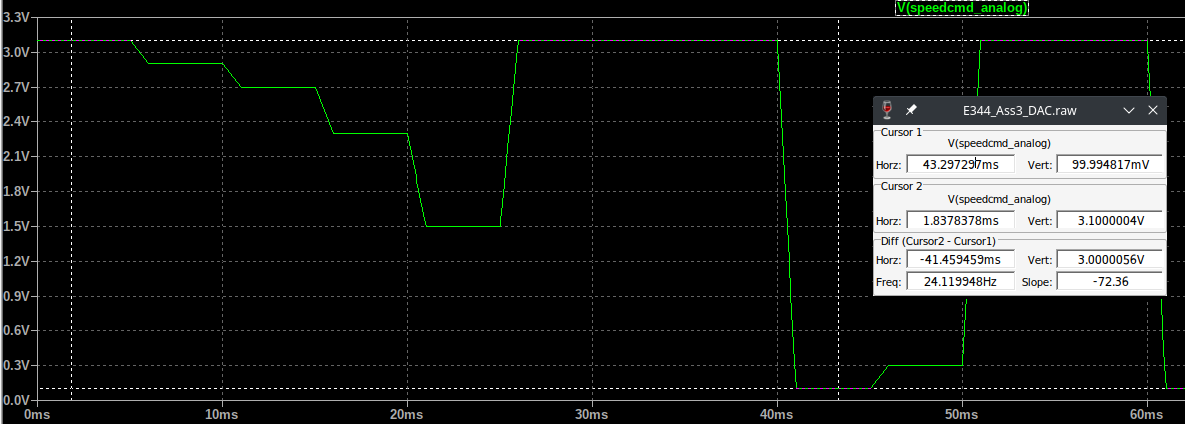
\includegraphics[width=1.0\linewidth]{dac_sim_range}
        \captionof{figure}{Output Range from 0000 (First Cursor) to 1111 (Second Cursor)}
        \label{fig:dac_sim_range}
    \end{minipage}
    \begin{minipage}{.45\textwidth}
        \centering
        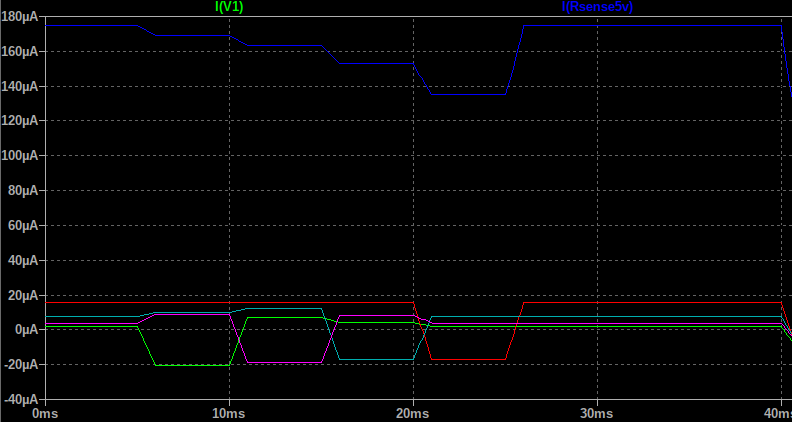
\includegraphics[width=1.0\linewidth]{dac_sim_currentDraw}
        \captionof{figure}{Current Draw (Amplifier and Digital Inputs)}
        \label{fig:dac_sim_currentDraw}
    \end{minipage}
\end{figure}

As seen in the above figures, all specifications were complied with:
\begin{itemize}
    \item Figure \ref{fig:dac_sim_range} shows that an output of 0000 produces exactly 3.1 V on the output, and that 1111 produces 100 mV.
    \item Figure \ref{fig:dac_sim_currentDraw} shows a maximum current draw of under $\SI{180}{\micro\ampere}$, which is much under the $\SI{250}{\micro\ampere}$ specification.
          It also shows that each digital input draws less than $\SI{20}{\micro\ampere}$, also under the $\SI{50}{\micro\ampere}$ specification.
\end{itemize}

\subsection{Measured}

\begin{figure}[!htb]
    \centering
    \begin{minipage}{.22\textwidth}
        \centering
        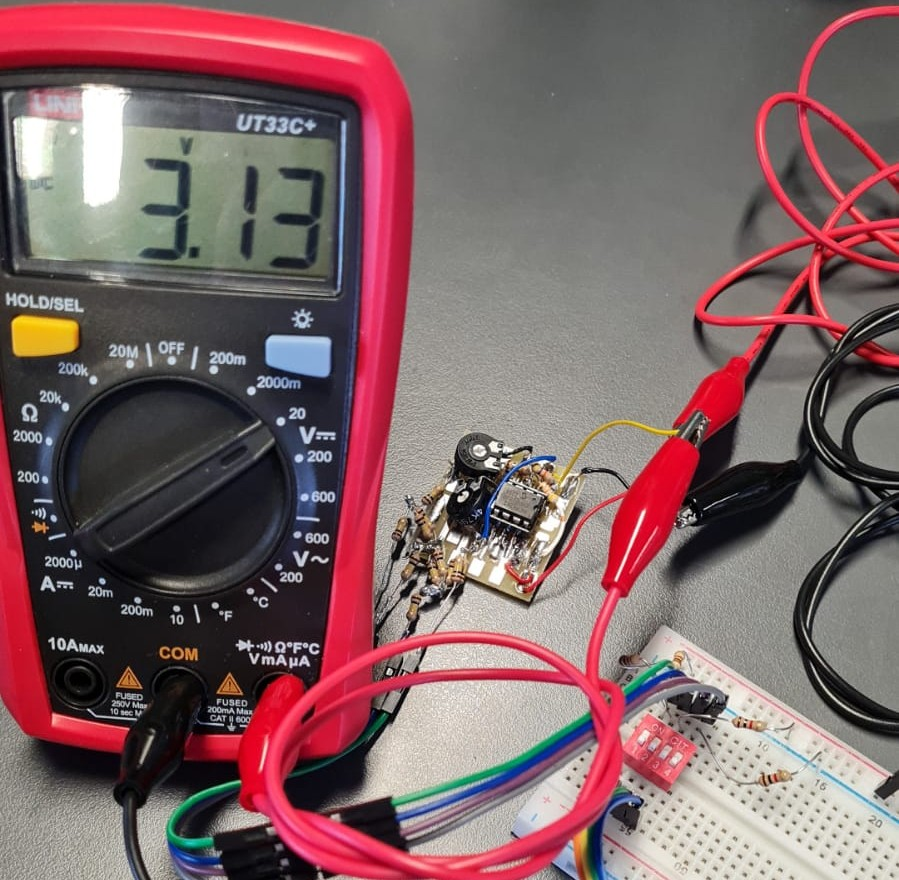
\includegraphics[width=1.0\linewidth]{dac_impl_0000}
        \captionof{figure}{DAC Output at 0000}
        \label{fig:dac_impl_0000}
    \end{minipage}
    \begin{minipage}{.2\textwidth}
        \centering
        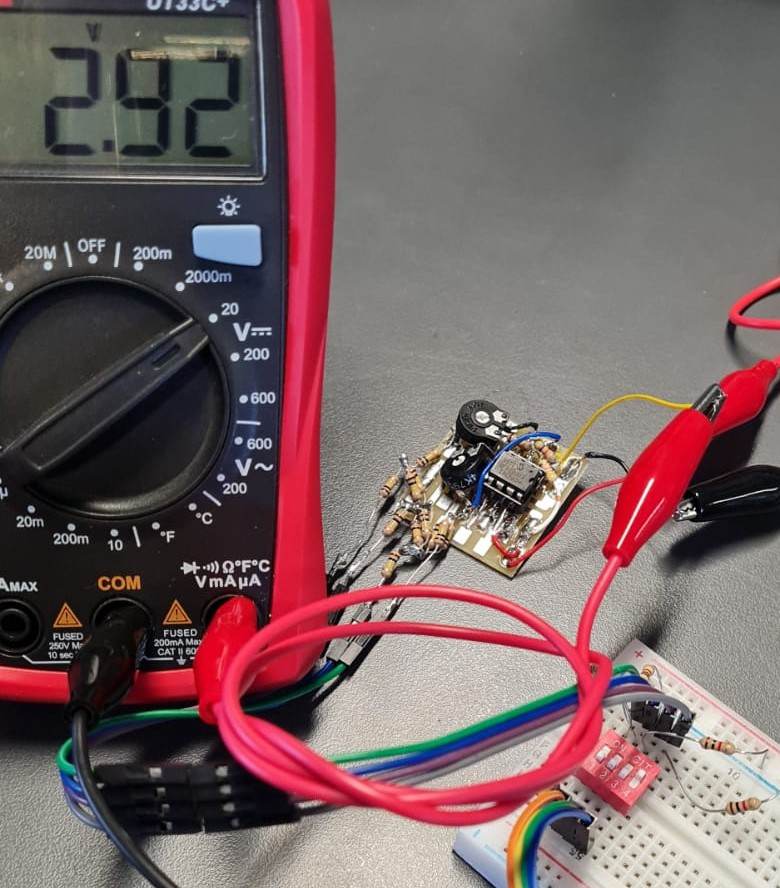
\includegraphics[width=1.0\linewidth]{dac_impl_0001}
        \captionof{figure}{DAC Output at 0001}
        \label{fig:dac_impl_0001}
    \end{minipage}
    \begin{minipage}{.22\textwidth}
        \centering
        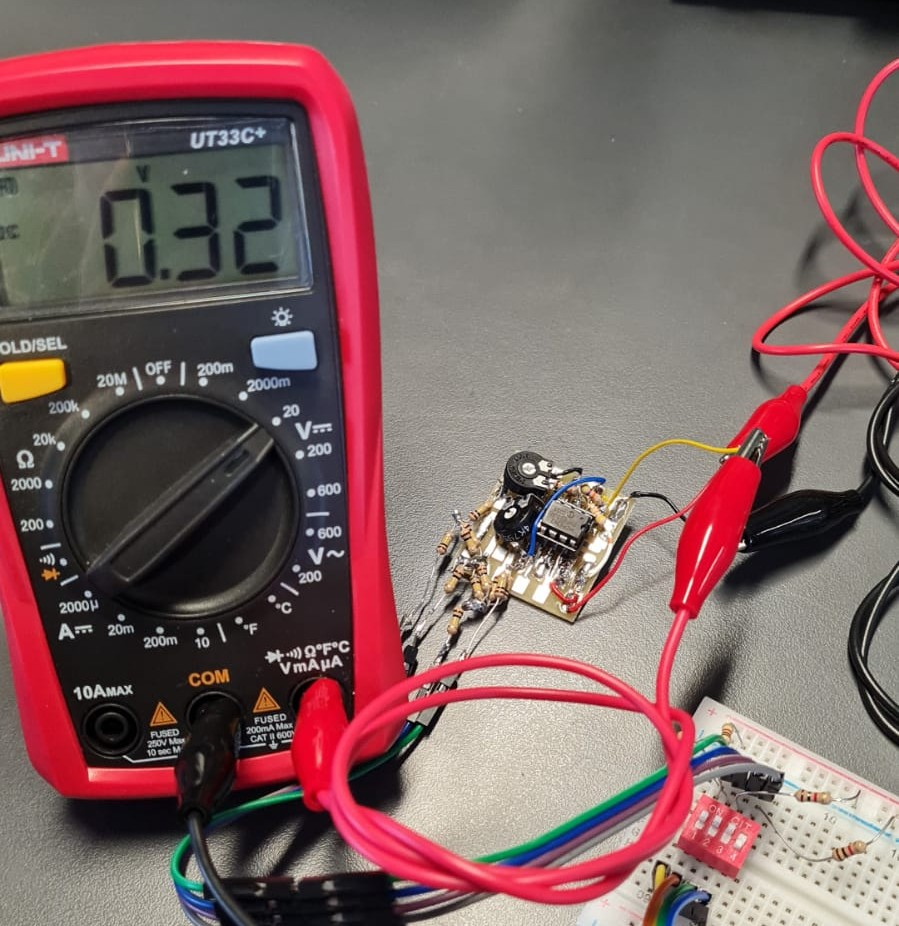
\includegraphics[width=1.0\linewidth]{dac_impl_1110}
        \captionof{figure}{DAC Output at 1110}
        \label{fig:dac_impl_1110}
    \end{minipage}
    \begin{minipage}{.2\textwidth}
        \centering
        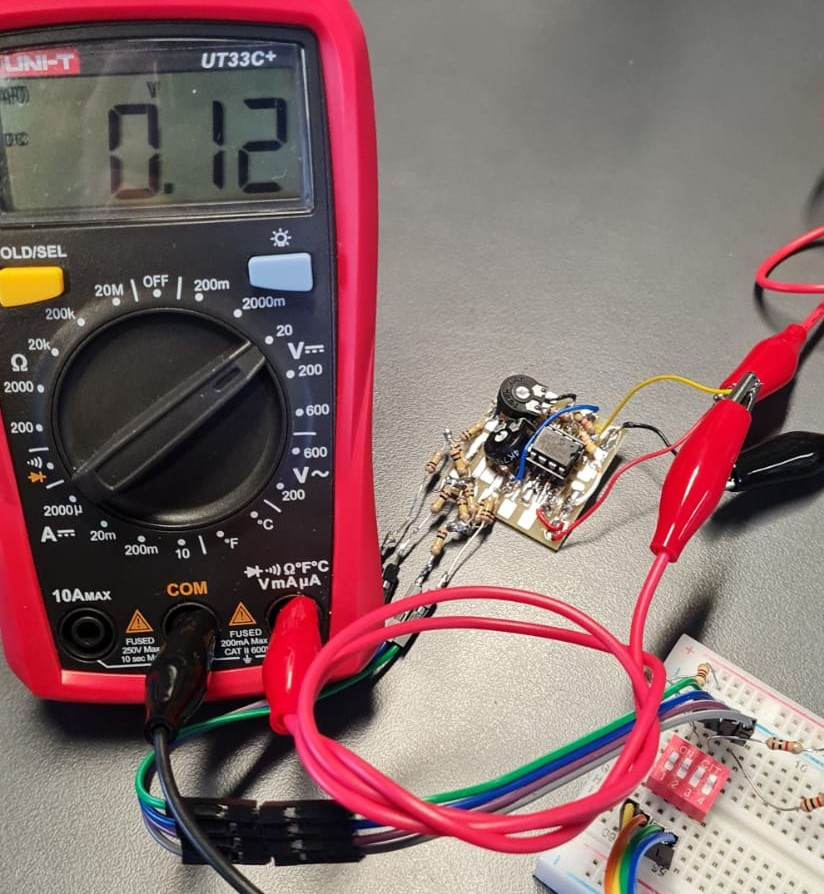
\includegraphics[width=1.0\linewidth]{dac_impl_1111}
        \captionof{figure}{DAC Output at 1111}
        \label{fig:dac_impl_1111}
    \end{minipage}    
\end{figure}

Figures \ref{fig:dac_impl_0000} to \ref{fig:dac_impl_1111} demonstrate the output voltages at specific digital input combinations.
All specifications are complied with, specifically that 0000 produces $> \SI{3}{V}$ on the output, and that 1111 produces $< \SI{0.5}{V}$.